\begin{figure}[htbp]
\centering
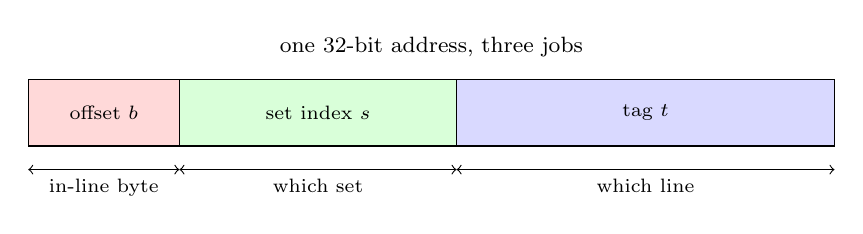
\begin{tikzpicture}[font=\footnotesize, x=3.2mm, y=6mm]
  \draw (0,0) rectangle (32,1.4);
  \draw[fill=red!15]  (0,0) rectangle (6,1.4);
  \draw[fill=green!15](6,0) rectangle (17,1.4);
  \draw[fill=blue!15] (17,0) rectangle (32,1.4);
  \node at (3,0.7) {\scriptsize offset $b$};
  \node at (11.5,0.7) {\scriptsize set index $s$};
  \node at (24.5,0.7) {\scriptsize tag $t$};
  \draw[<->] (0,-0.5) -- (6,-0.5) node[midway,below]{\scriptsize in-line byte};
  \draw[<->] (6,-0.5) -- (17,-0.5) node[midway,below]{\scriptsize which set};
  \draw[<->] (17,-0.5) -- (32,-0.5) node[midway,below]{\scriptsize which line};
  \node at (16,2.1) {one 32-bit address, three jobs};
\end{tikzpicture}
\caption{The address split: \texttt{tag} picks the line inside the
set, \texttt{index} picks the set, \texttt{offset} picks the byte
within the 64-byte line. Every cache geometry question reduces to
where these boundaries fall.}
\label{fig:split10}
\end{figure}
